\documentclass[
  twoside,
  12pt, a4paper,
  footinclude=true,
  headinclude=true,
  cleardoublepage=empty
]{article}
\usepackage[utf8]{inputenc}
\usepackage{color}
\usepackage{mathtools}
\usepackage{graphicx}
\usepackage{hyperref}
\hypersetup{urlbordercolor={1 1 1}}


\begin{document}
The Structure of the thesis
\begin{enumerate}
    \item[1.] Motivation
        \begin{enumerate}
            \item[1.1] Python language overview
            \item[1.2] R language overview
            \item[1.3] Python vs R wars
            \item[1.4] Thesis description
            \item[1.5] Data preparation 
        \end{enumerate}
    \item[2.] Python
        \begin{enumerate}
            \item[2.1] The structure of the program
            \item[2.2] The process description
            \begin{enumerate}
                \item[2.2.1] Used Libraries
                \item[2.2.2] Documentation quality and quantity
                \item[2.2.3] Advantages and disadvantages of the program 
            \end{enumerate}
            \item[2.3] Results
        \end{enumerate}
    \item[3.] R
        \begin{enumerate}
            \item[3.1] The structure of the program
            \item[3.2] The process description
            \begin{enumerate}
                \item[3.2.1] Used Libraries
                \item[3.2.2] Documentation quality and quantity
                \item[3.2.3] Advantages and disadvantages of the program 
            \end{enumerate}
            \item[3.3] Results
        \end{enumerate}
    \item[4.] Results
        \begin{enumerate}
            \item[1.1] Objective comparison
            \item[1.2] Subjective comparison
            \item[1.3] Conclusion
        \end{enumerate}
    \item[5.] Literature
\end{enumerate}

\newpage
\section{Motivation}
Nowadays, with the massive digitalization of the world, statistical analysis is used almost everywhere. Along with the classical fields of data analysis such as production, logistics, marketing and so on, new spheres like e-commerce and video gaming require statistical analysis to succeed. In order to create a professional web site to attract customers and more important to make them purchase things from this particular online shop, a customer behavior analysis is required as well as an analysis of the product. The video gaming industry can be another example of the sphere where data analysis is essential for success. The AI in a game (NPC or event generator) constantly analyzes the incoming data from the players, servers and third party sources to improve its performance. The game play, the enemies, the load distribution on the servers and many other things are adjusted accordingly to the results of the constant data analysis and predictions. These are only several examples where statistical analysis plays an important role but there are many others. Almost every aspect of modern life is connected with data analysis.\vspace{3mm}\\
Since the computer technologies are way more advanced than they were several decades ago, many different approaches, tools and frameworks are available for automatized computations as well as for an automatized data collection. However, for every purpose, a certain set of tools, languages and libraries should be carefully chosen. In this work we will concentrate our attention on using two very popular languages to solve a simple statistic-econometric task. Almost every modern programming language can be used to build a program for collecting, processing and visualizing data: SCALA, C, C++, .NET, Java, Python, JavaScript.\vspace{3mm}\\
In this work we will concentrate on two popular programming languages. We will compare Python 3 with R. Both of them are fairly recent (Python is about 25 years old and R is about 22 years old). Both languages are widely used for data analysis and are commonly employed in open source projects. They both have large communities behind them. An important factor for this work was each languages' respective learning curve. Statistic programs in this work will be written in beginner style. Python and R are relatively easy to begin with even for non-programmers. Python has a gradual learning curve due to its simplicity, clear and intuitive syntax. Although R has a steep learning curve, beginners still can use it pretty easy for up to moderately complex projects.

\newpage
\subsection{Python language overview}
The first public release of Python was 24 years ago. Python is a general-purpose, high-level programming language. Its design philosophy emphasizes code readability and its syntax allows programmers to express concepts in fewer lines of code than would be possible in languages such as C++ or Java.[21][22] The language provides constructs intended to enable concise programs on both a small and large scale [1]. That means that Python can be used for many tasks like back end development, front end development, data analysis and even for processor simulation. The language supports multiple programming paradigms: object oriented, imperative and functional programming.\\ 
The Python language has an automatic garbage collector.\\
The community behind Python is very large which results in many different official libraries and packages as well as the third party tools. The standard library contains many packages sufficient for an easy start. The language's syntax is clear in comparison to C++, C or even Java.\\
Another important factor for why Python was chosen for this work is its build
t-in doctest module. This module is easy to use for checking and debugging the codes logic. The biggest advantage of the doctest for beginner programmers is that doctest's code is written inside of the program code. Unit tests are also widely used among the Python programmers. There are also other possibilities to debug and benchmark the code written in Python but we will not discuss it in this work.\\

\subsection{R Overview}
R is a programming language and software environment for statistical computing and graphics. The R language is widely used among statisticians and data miners for developing statistical software and data analysis. Polls, surveys of data miners, and studies of scholarly literature databases show that R's popularity has increased substantially in recent years [5]. R is a successor of the S language, proposed about 39 years ago. R is distributed under GNU General Public license which makes this language a suitable choice for open source analytical projects.\\
Same as Python, R also uses an interpreter to execute the code. R is a single-purpose language. The main use of R is statistical analysis and visualization. Since R is an open source project, there is also a big community behind it. The community behind R language is of mostly scientific nature.\\
The disadvantage of R is its single-purpose nature. The use of such project will be reduced, since there are few quick and comfortable ways to integrate the program into a real system.\\

\subsection{Python vs R wars}
Since both languages offer tons of packages and libraries for analyzing and visualization, people argue about what language is a better fit [6],[7],[8],[9],[10].
So far nobody has managed to give a satisfactory final answer, since the languages indeed are different. The answer will differ depending on task scale, complexity, requirements. A viable strategy is providing a list of requirements with points for each requirement for every concrete task and scale. This way it is possible to compare the languages more or less objectively without letting the subjective judgment and preferences make the evaluation biased.\\
In this work we have developed our own list of criteria to compare Python and R. This list contains following points:
\begin{enumerate}
    \item The amount of useful resources for the task.
    \item Clear documentation with examples.
    \item Performance.
    \item Memory use.
    \item Appropriate data structures.
    \item Possibility to work with Big Data.
    \item Visualization tools.
    \item Hard or soft limitations.
    \item Need for workarounds.
\end{enumerate}
Using this list, both languages can be objectively evaluated. These points were chosen to be appropriate for all small, middle and enterprise-level projects. In the next section we will describe the test-task to compare Python and R languages and define the points system for objective evaluation.\\

\subsection{Thesis Description}
The idea of this bachelor thesis is to test which of the languages is more suitable for specific statistic task. Both programs will have similar structure and functions, so that they can be evaluated more properly. The program that will be evaluated consists of four parts:
\begin{enumerate}
    \item Getting and formatting data - the program should be able to read a prepared file in csv format. Afterwards, the program should format the data into needed structure for further use.
    \item Analyzing data - the program should be able to run statistical tests to figure out several data characteristics. This step is implemented in order to determine what regression models are allowed for this data set. The following tests will be presented: stationary test, building cdf and kde, finding moments, distribution test (goodness of fit tests).
    \item Building a model - the program should be able to create a proper model using a step-forward algorithm. The preparation step is creating a correlation vector and leaving out all companies with the correlation coefficient smaller than 30\%. As the first step the limits on the number of the predictors in the final regression will be set. The second step is to create a one parameter model using the correlation vector (take the company with the highest correlation coefficient). The third step is iterative model building: 
    \begin{enumerate}
        \item Create all possible double combinations consisting of fixed company name from the previous step and not used company name. Choose the best multiple linear regression built with GLS method among the class. 
        \item Compare two models from different classes using LLR test.
        \item If the smaller model is better, the search is over, the program returns the result.
        \item If the bigger model is better, the iteration continues until the smaller model will be better or the limit on the parameters in the regression is reached. The program then returns the result. 
    \end{enumerate}
The output of the program shows the names of the companies in the final regression, main statistics, coefficients.
    \item Visualization - the program should be able to present the results in the form of graphs for needed steps.
    \item The program is able to build predictions for the chosen company and evaluate them using the mean accumulated error (MAE) and or root-mean-square error (RMSE).
\end{enumerate}
The program will build a simple regression if possible. In this work we have considered the class of linear regressions to be a simple regression model. This task is considered to be middle-size task, not too easy but at the same time not too time consuming and specific.
The data will be prepared and provided by two files: training set and test set in the csv format.\\
According to the list for objective evaluation, each point will give either a score of 0 or 1 to the language. A score of 0 will be given in negative case and a score of 1 will be given in positive cases.
\begin{enumerate}
    \item[] Useful resources - at least 2 different libraries for one task gives 1 point.
    \item[] Documentation - examples, clean source code and clear structured APIs give 1 point.
    \item[] Performance - fastest language gets 1 point
    \item[] Memory - the program with the smallest memory use gets 1 point.
    \item[] Data structures - no additional formatting needed gives 1 point.
    \item[] Big Data - libraries, plugins and frameworks for big data give 1 point.
    \item[] Visualization - easiness in use and customization gives 1 point.
    \item[] Limitations - if there are any limitations, the language gets 0 points.
    \item[] Workarounds - additional time to solve the task gives 0 points (deviation from the time for the naive implementation).
\end{enumerate}
The results of the programs will be also compared. If they differ, the models will be cross-compared.\\
The task is to build a best matching linear regression (if possible) for a company (always the first column in the file) using certain limitations on the number of the predictors.

\subsection{Data preparation}
The data set for this work will be prepared in advance. For our purpose we decided to take Intel as a dependent variable in the regression. Predictors will be chosen among the companies from the same market of micro controllers, supplier market and customers market. We have chosen Intel because it is a transparent diversified company with clear development trend this company is one of the leaders ob the microchips market and all connected markets are also easy to define. In this work we will consider only a small amount of companies influencing Intel, since we want to keep the task on medium complexity.\\
Intel's competitors can be found on Wikipedia listed in several tables for years from 1998 to 2013. We have used a parser to get the following list of manufacturers for the years 2000-2013 for semiconductors market:
\begin{verbatim}
['AMD', 'Qualcomm', 'Micron Technology','Hynix',
'Infineon Technologies', 'Intel Corporation', 
'STMicroelectronics', 'Texas Instruments']
\end{verbatim}
Semiconductors are the basic component for different devices, so the potential consumer-markets may vary. In this bachelor thesis we will concentrate on microchips (CPUs) consumers. The following consumer markets are: tablets, smartphones, personal computers, automobiles, video game consoles, medical technologies, engineering technologies, aviation. Tablets and personal computers are united into one market-group.\\
Automobile market:
\begin{verbatim}
['Toyota', 'GM', 'Volkswagen', 'Ford', 'Nissan', 
'Fiat Chrysler Automobiles', 'Honda', 'PSA', 'BMW',
'Daimler AG', 'Mitsubishi', 'Tata', 'Fuji']
\end{verbatim}
The only significant players (manufacturers) on the gaming console market are: Microsoft, Sony and Nintendo.\\ 
The aviation market is presented by the following companies: 
\begin{verbatim}
['Boeing', 'United Technologies', 'Lockheed Martin',
'Honeywell International', 'General Dynamics',
'BAE Systems', 'Northrop Grumman', 'Raytheon',
'Rolls Royce', 'Textron', 'Embraer', 'Spirit AeroSystems Holdings Inc.']
\end{verbatim}
The next microchips consumer markets are smartphones, tablets and PCs markets. Since many companies are presented on the markets mentioned above and have further production markets, we will put them into "Diversified" category. The diversified companies that may influence Intel are:
\begin{verbatim}
['Samsung', 'Apple', 'Microsoft', 'Nokia', 'Sony', 'LG',
'Motorola',  'Lenovo',  'BlackBerry', 'Alcatel', 'Vodafone']
\end{verbatim} 
Another huge consumer market for Intel is the medical equipment market. The following companies present this sphere:
\begin{verbatim}
['Johnson & Johnson', 'General Electric Co.', 'Medtronic Inc.',
'Siemens AG', 'Baxter International Inc.', 
'Fresenius Medical Care AG & Co.', 'Koninklijke Philips',
'Cardinal Health Inc.', 'Novartis AG', 'Stryker Corp.',
'Becton, Dickinson and Co.', 'Boston Scientific Corp.',
'Allergan Inc.', 'St. Jude Medical Inc.', '3M Co.',
'Abbott Laboratories', 'Zimmer Holdings Inc.', 
'Smith & Nephew plc', 'Olympus Corp.', 'Bayer AG',
'CR Bard Inc.', 'Varian Medical Systems Inc.',
'DENTSPLY International Inc.', 'Hologic Inc.', 
'Danaher Corp.', 'Edwards Lifesciences', 'Intuitive Surgical Inc.']
\end{verbatim}
Additionally to the companies mentioned above, several big players from the industrial equipment market will be added. These are the following companies:
\begin{verbatim} 
['ABB Robotics', 'Adept Technology', 'Bosch', 'Caterpillar',
'Denso Robotics', 'Google', 'Universal Electronics']
\end{verbatim}
After limiting the number of the connected markets, we have limited the number the companies from the chosen markets, because of the lack of the information about some companies. The reason for the lack of information is that some companies have entered the international stock exchange recently (since 2010 earliest). Some companies are still closed for foreign investors (which is the case for giants such as Samsung, Honda and other Asian companies). The last limit on the chosen companies is the trading volume. If  the trading volume for the last two years were zero, the company was considered to not have been traded on the stock exchange.\\
After the companies were chosen, the whole data table was split into two data sets: learning set and validation set. We have obtained daily prices from 2006 to 2015 (31.12.2014 is the last date for all indexes). The training or learning set will be approximately 70\% of the whole data volume: from 2006 to 2010. The validation set is about 30\%: from 2011 to 2012. For this work we use the daily frequency (only opening prices).\\

\newpage
\section{Python}
\subsection{The structure of the program}
The program consists of three functional classes, connected with each other in the main class. The first class is called DataFormating and it is responsible for getting the data out of the csv file and writing it into an instance of a proper format for the other two classes. The dependent variable will be extracted from the data set (the dependent variable is always the first company listed in the first column in the csv table).\\
The second class is called StatisticTests. It runs several tests to find out the main static characteristics in order to choose an appropriate model class for the data. In this work we have focused on the linear regression class.\\
The third class is called BuildModel. This class builds the multiple linear regression (according to the results of the StatisticTests class) using the step-forward approach:
\begin{enumerate}
    \item The amount of companies taken into account is reduced using the correlation vector: all companies having the correlation coefficient less than 30\% are omitted.
    \item A limit on the maximum number of the parameters is set using the following rule: 1 company out of 10 if the number of companies exceeds 5.
    \item The first step is to find the best one-parameter model using the highest correlation coefficient from the first step.
    \item All possible combinations for fixed companies from the previous step and remaining companies are created. For all these combinations the linear regression using Generalized Least Squares approach [24] is built.
    \item The best model among the class is chosen using the AIC criterion.
    \item Best models among the classes are compared using the likelihood ratio test. 
    \item If the bigger model is better and the limit of the predictors in regression is not achieved, the new small model is set to be equal to the old bigger model. The whole computations are repeat from step 4. The final result is equal to the last bigger model.
    \item If the smaller model is better or the maximum number of parameters in the final regression is achieved then the final result is either the small model or the last big model. 
\end{enumerate} 
At the end the program returns the names of the companies in the final regression and the full information for the best model.

\subsection{The process description}
In this section we will describe the language specific difficulties we have encountered.
\subsubsection{Libraries Used}
In the course of writing the program several steps were implemented. These steps are: extracting and preparing the data for further use, checking statistic characteristics and building the model based on the results of the statistics. In order to build the program three main libraries were used:
\begin{enumerate}
    \item Python Standart Library [12].
    \item SciPy (unites six different libraries) [13].
    \item Statmodels [14].
\end{enumerate}
The functions and the data structures defined in the standard Python library were used for every simple task, except some mathematical computations, since the NumPy library offers faster implementations.\\
The second most used library in this work was NumPy. This library is the part of the SciPy source. NumPy offers many fast multi-dimensional computations and associated multi-dimensional structures. In our work we have used this library to compute several statistics and to build the data for displaying graphs. The functions in the standard library did not show the sufficient performance needed for our program:
\begin{verbatim}
>>> x=[random.randint(0,10) for i in range(0,1500)]
>>> len(x)
1500

>>> mean_base = statistics.mean(x)
>>> mean_base
4.966
>>> cProfile.run('statistics.mean(x)')   
         4531 function calls in 0.006 seconds
        
>>> mean_numpy = numpy.average(x)
>>> mean_numpy
4.9660000000000002
>>> cProfile.run('numpy.average(x)')
         17 function calls in 0.001 seconds
\end{verbatim}   
As you can see, the NumPy implementation of the function average yields more accurate results and better performance. The run time difference can be already shown on the data list containing 1500 integers.\\
The third important library used in this work is Pandas. The library is a part of the SciPy source. Pandas provides the high-performance data structures and associated functions for data analysis. This library can be used for generating, accessing and formatting data. In this work we have used it to get the data from our csv file in an intuitive manner and also to avoid an unnecessary formatting step. Pandas offers the functionality to get the data directly from web sources like Yahoo Finance, Google Finance, Google Analytics and other similar sources. We didn't use this functionality in our program since our task did not require the up-to-date data and we did want to save the possibility to correct the csv file manually if needed. Another possible problem using the data directly from the web is the necessity of a more complex program to cut off the data when the trading volume was null.  The following method return data.frame object that is formatted later on for further use.
\begin{verbatim}
>>> data = pd.read_csv(str(self.file_name))
>>> cProfile.run('data = pd.read_csv("../data/LearningSet.csv")'
        3316 function calls (3238 primitive calls) in 0.024 seconds
\end{verbatim}
The LearningSet file is a table containing 78 companies with 1240 prices for each company. The total size of the table is approximately 500KiB.\\ The library for drawing graphs is called Matplotlib. It is also a part of the SciPy source. Matplotlib offers different types of graphs and formatting tools. The following example represents the default graph without any additional formatting.
\begin{verbatim}
>>> plt.title(3M)
>>> plt.plot(bin_edges[1:], cdf)
>>> plt.clf()
\end{verbatim}
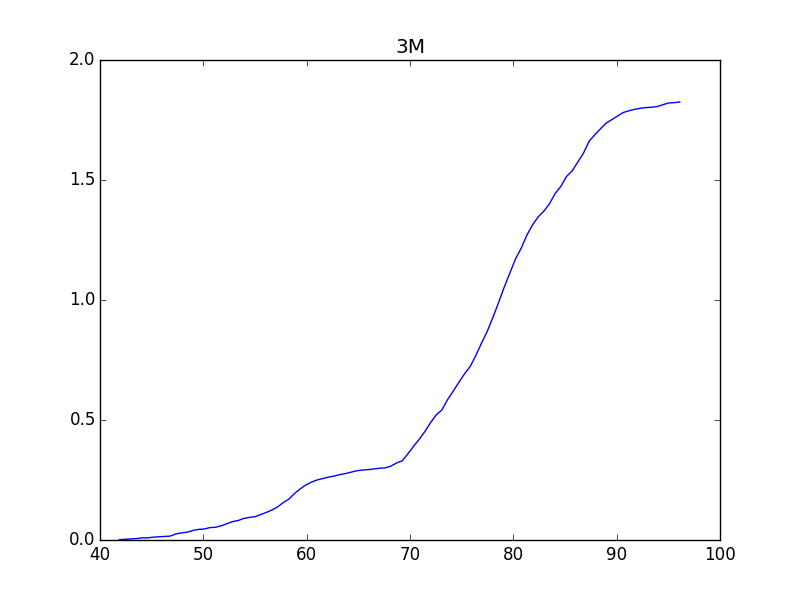
\includegraphics[scale=0.75]{PythonPlotExample.png} \\
The last library is called Statmodels. This library offers a variety of tools and models for statistic purposes. The main functions of the library used in our program are: Augmented Dickey-Fuller test and building a multiple linear regression with generalized least squares approach.
\begin{verbatim}
>>> statistic = statmodel.adfuller(self.dict_data[key], 250, 
                        'ctt', 't-stat', False, False)[0] - stationary test
                        
>>> model_null = sm.GLS(y, smaller_model_list)
>>> info_small_model = model_null.fit().summary()
\end{verbatim}   

\subsubsection{Documentation quality and quantity}
The quality and the quantity of the documentation plays an important role for the project of every complexity. In this work we will evaluate the documentation of the languages using a score system. Each language will get points for the following criteria described in the table below:
\begin{enumerate}
    \item The documentation is always available.
    \item The documentation is easy to navigate.
    \item The documentation offers a sufficient amount of examples.
    \item The examples given in the documentation cover different complexity levels.
    \item The documentation provide a link to the source code.
    \item For scientific libraries the theoretical background should be provided.
    \item The documentation is easy to read (formatting, colors, description of the parameters and output).
\end{enumerate}
Originally, Python was used a lot for scientific purposes. This is why many libraries have specific formatting and high complexity. As we have already mentioned earlier, in this work we have used Python 3 standard library [12],  SciPy [14] and Statmodels [15].\\
The Python program was written in Python 3. In our work we did not encountered any problems with the language versions conflict. Some external libraries can only be compatible with the Python 2. For such conflicts the library called Six [16] can be used.\\
According to the provided evaluation table all used libraries will get points and the weighted score will be added to the python total score. The weights are approximate and are based on appearance frequency and importance of the library in the program.\\
The base Python library:
\begin{enumerate}
    \item 1 Point (the documentation was always available, no delays over period of 6 month were noticed).
    \item 1 Point (the web site is modern and has a clear structure).
    \item 1 Point (each function has one simple example, some functions are explained by an "identical function" example, at the end of the class description several composite examples are given).
    \item 1 Point (see above).
    \item 0 Point (the code is can't be accessed freely).
    \item 1 Point (functions are either explained in the documentation, or provide a link to an external source).
    \item 1 Point (the documentation structure is same for every class. The Navigation through the documentation is possible using global index, glossary, etc.).
\end{enumerate}
From the SciPy source three libraries were used explicitly:
. These are NumPy, Matplotlib and Pandas. The documentation of the libraries themselves contains more detailed information and some additional examples, but the structure and the formatting are the same according to the Python styling standard. This is why we will evaluate the SciPy documentation instead of evaluating each library.
\begin{enumerate}
    \item 1 Point.
    \item 1 Point.
    \item 1 Point.
    \item 1 Point.
    \item 1 Point.
    \item 1 Point.
    \item 1 Point.
\end{enumerate}
The most important library for our Python program was Statmodels since we used it to build the models.
\begin{enumerate}
    \item 0 Point (the documentation is hosted on the Sourceforge and the server was down for about a week during the program development phase).
    \item 0 Point (the structure is not clear, dependencies are not intuitive).
    \item 1 Point.
    \item 0 Point (basic examples are not always provided by the documentation).
    \item 1 Point (the source code is hosted on GitHub).
    \item 1 Point.
    \item 0 Point (the explanation order of the input parameters, output parameters and methods is alphabetical and not logical).
\end{enumerate}
The final score for the Python documentation is:
\[ \frac{(\frac{2}{5}(6) + \frac{1}{5}(7) + \frac{2}{5}(3) )}{7}= 0.71\]


\subsubsection{Advantages and disadvantages of the program}
During the program development phase we have encountered several langauge specific advantages and disadvantages.\\
The first advantage is the small time investment needed up front. Python is intuitive and does not require deep understanding of the programming paradigm for a simple program. We consider Python to be suitable for prototyping and checking small hypothesis.\\
The second advantage of the language is testing. Python has a built-in doc-tests [22]. Another possibility to test a program are Unit Tests [23]. Python provides different ways to test and to debug the program in order to avoid possible computational and logic errors. We will not discuss this theme in details since the tutorials and the documentation are simple and offer sufficient amount of examples.\\
There are several disadvantages of the statistic program written in Python.\\ 
The first disadvantage is the performance. This disadvantage can appear mostly for beginners by implementing middle complexity tasks. For large data sets Cython might be used instead of simple Python.\\
The main time consumption comes from StatisticTests. 
\begin{verbatim}
>>> cProfile.run("statistics.stationarity()")
        2898213 function calls (2887173 primitive calls) in 5408.838 seconds
\end{verbatim}
In order to avoid data formatting difficulties we have used Pandas library. There are some limitations of the library, it is not compatible with the PyPy3. This is why our program couldn't have been sped up easily.\\
Another disadvantage of the program written in Python is the time you have to invest into the language investigation for more the tasks of the higher complexity. There are several non-intuitive functions and data structure uses.
\begin{verbatim}
>>> a = {"a":[1,2,3], "b":[1,2,3], "c":[1,4,9]}
>>> b = a
>>> b["a"] = [1,4,9]
>>> b
{'b': [1, 2, 3], 'a': [1, 4, 9], 'c': [1, 4, 9]}
>>> a
{'b': [1, 2, 3], 'a': [1, 4, 9], 'c': [1, 4, 9]}
\end{verbatim} 
Python does not implicitly creates copies. The example above shows how two objects are referred to the same object. During mutating one of the objects all references will change in order to keep referring to the object in its current state. The proper way to use dictionary is described below:     
\begin{verbatim}
>>> a = {"a":[1,2,3], "b":[1,2,3], "c":[1,4,9]}
>>> b = a.copy()
>>> a
{'b': [1, 2, 3], 'a': [1, 2, 3], 'c': [1, 4, 9]}
>>> b
{'c': [1, 4, 9], 'b': [1, 2, 3], 'a': [1, 2, 3]}
>>> b["a"] = [0]
>>> b
{'c': [1, 4, 9], 'b': [1, 2, 3], 'a': [0]}
>>> a
{'b': [1, 2, 3], 'a': [1, 2, 3], 'c': [1, 4, 9]}
\end{verbatim}
or 
\begin{verbatim}
>>> a = {"a":[1,2,3], "b":[1,2,3], "c":[1,4,9]}
>>> b = dict(a)
>>> b
{'c': [1, 4, 9], 'b': [1, 2, 3], 'a': [1, 2, 3]}
>>> b["a"]=[0]
>>> b
{'c': [1, 4, 9], 'b': [1, 2, 3], 'a': [0]}
>>> a
{'b': [1, 2, 3], 'a': [1, 2, 3], 'c': [1, 4, 9]}
\end{verbatim}
The last disadvantage we want to mention is the unsorted nature of the dictionary. After the csv table was read and formatted into dictionary with the companies names as the keys and the associated prices lists as the values. The keys appear in dictionary in random order. In order to get the name of the first column in the table following command can be used:
\begin{verbatim}
>>> d = {"a":[1,2,3,4], "b":[3,1,2,4], "c":[1,5,1,2]}
>>> d.keys()
dict_keys(['a', 'c', 'b'])
>>> sorted(d.keys())
['a', 'b', 'c']
\end{verbatim} 

\subsection{Results}
The end result is printed out to a console. The final message contains the names of the companies used in the final regression, main characteristics of the regression (AIC, BIC, Loglikelihood, coefficients and errors) and the total run time of the program. 
The results of the program for the given data described in the data preparation section are:
\begin{verbatim}
The best model contains  6  parameters. And the model is:
['STMElectro', 'Olympus', 'St Jude', 'Lenovo', 'MicronTech', 'Google']
                            GLS Regression Results                            
==============================================================================
Dep. Variable:                      y   R-squared:                       0.998
Model:                            GLS   Adj. R-squared:                  0.998
Method:                 Least Squares   F-statistic:                 8.701e+04
Date:                 Do, 24 Sep 2015   Prob (F-statistic):               0.00
Time:                        20:20:45   Log-Likelihood:                -1753.3
No. Observations:                1239   AIC:                             3519.
Df Residuals:                    1233   BIC:                             3549.
Df Model:                           6                                         
Covariance Type:            nonrobust                                         
==============================================================================
                 coef    std err          t      P>|t|      [95.0% Conf. Int.]
------------------------------------------------------------------------------
x1             0.1254      0.016      7.933      0.000         0.094     0.156
x2             0.0609      0.012      5.065      0.000         0.037     0.085
x3             0.3261      0.016     21.029      0.000         0.296     0.357
x4             0.2126      0.004     47.272      0.000         0.204     0.221
x5             0.0083      0.001     12.929      0.000         0.007     0.010
x6             0.1291      0.012     10.536      0.000         0.105     0.153
==============================================================================
Omnibus:                       10.831   Durbin-Watson:                   0.120
Prob(Omnibus):                  0.004   Jarque-Bera (JB):               10.859
Skew:                           0.212   Prob(JB):                      0.00439
Kurtosis:                       2.827   Cond. No.                         357.
==============================================================================

[Finished in 4173.2s]
\end{verbatim}
To sum up the objective arguments for Python program computing a linear regression for a given data and restrictions we will sum up the points from the table from the thesis description section.
The points for the Python program are:
\begin{enumerate}
    \item Useful sources: 1 Point.
    \item Documentation: 0.71 Point.
    \item Performance: 0 Points.
    \item Memory: 0 Points.
    \item Uniform Data structures: 0 Points (different libraries uses different shapes).
    \item Big Data: 1 Point.
    \item Visualization: 1 Point.
    \item Limitations: 1 Point.
    \item Workarounds: 1 Point.
\end{enumerate} 
The Python program gets 5.71 points in total.\\
The subjective arguments for and against are: 
\begin{enumerate}
    \item The syntax is simple.
    \item The data structures are the same as you imagine.
    \item Slicing of the data arrays is intuitive.
    \item For small data arrays the performance of the language is sufficient.
    \item Debugging messages are easy to understand.
\end{enumerate}  

\newpage
\section{R}
\subsection{The structure of the program}
In this work we have written the R program the same way as the Python program. The R program consists of three classes. These classes are DataFormatting, StatisticTests and BiuldModel. The functions of the classes  are similar to the functions from the Python program. There are several language specific differences. The main class is implemented in the from of two separate functions. Since we wanted to gain more control over the program flow all functions and imported classes were called via console in R run time.\\
R is a convenient language in terms of data formatting. The native method read.csv() returns an object called data frame. This object has differebt methods allowing to use the data from different spots in the program directly without extracting it and saving in a proper format. For example, the list of all companies from the table was extracted using the function colnames(data.frame). As an output we have got the list object containing the elements from the first row of the table. The R program does not have inner helpers as the Python program.\\
The class StatisticTests runs tests to detect statistic characteristics of the data. These tests contain Kolmogorov-Smirnov goodness of fit distribution test, Augmented Dickey-Fuller test, building a cumulative distribution function and a kernel density function, finding moments.\\
The third class called BuildModel creates the multiple linear regression for  the given data table. The procedure of the regression building is the same step-forward approach that was implemented in the Python program:
\begin{enumerate}
    \item Cut off all companies with the correlation coefficient smaller than 30\%.
    \item Set the limit for the maximum number of parameters in the final regression. 
    \item Choose the best one-parameter model.
    \item Build all possible combinations consisting of fixed companies from the previous steps and one unused company.
    \item Choose the best model among the two-parameter model class.
    \item Compare the best models from two different classes uing the Likelihood Ratio Test.
    \item Repeat until either the smaller model will be better, or the maximum number of parameters is reached.
\end{enumerate}

\subsection{The process description}
In this section we will describe the language specific difficulties we have encountered.
\subsubsection{Used Libraries}
For our R program following packages were used:
\begin{enumerate}
    \item Base package[16].
    \item Stats package[17].
    \item Nlme package[18].
    \item Tseries package[19].
\end{enumerate}
The functions from the base package were used for all basic computations. This package also provides different functions for the data formatting. The following example shows the R specific object called formula:
\begin{verbatim}
formula <- as.formula(paste(dep$name,"~", as.character(names(small_model)), collapse=""))
\end{verbatim}
This function converts the string object from the brackets into a formula object that is further used as an input parameter for building a linear regression. The base package offers basic math operation as well.\\
The StatisticTests class uses both stats and tseries packages to build the statistic tests on the data. The tseries package offers different tests and methods widely used in the computational finances and time series analysis. In this work we have only used Agumented Dickey-Fuller test to check the data for stationarity:
\begin{verbatim}
test <- adf.test(data[[company]])
\end{verbatim}
The second package used in StatisticTests class offers functions to run simple statistic tests on the data and build the basic statistic characteristics and provides the possibility to build a graph. In our work we have used the stats package to build graphs for each company from the data table and test the data for its distribution. The program has yielded the same results as the Python program.\\
The fourth package used in this program offers a possibility to build a linear regression using given parameters. The use of the functions from the library are intuitive:
\begin{verbatim}
small <- gls(as.formula(paste(dep$name,"~", as.character(names(small_model)), collapse="")), data)
\end{verbatim} 
The first parameter is formula object. The example of the this particular object we have already demonstrated above. The second parameter is the data source. A necessary condition for the data object is actually to contain the variables from the formula.\\
The following example presents a graph built without additional formatting:
\begin{verbatim}
png(path_cdf)
plot(graph[[name]], verticals = TRUE, do.points = FALSE, main=name)
dev.off()
\end{verbatim}
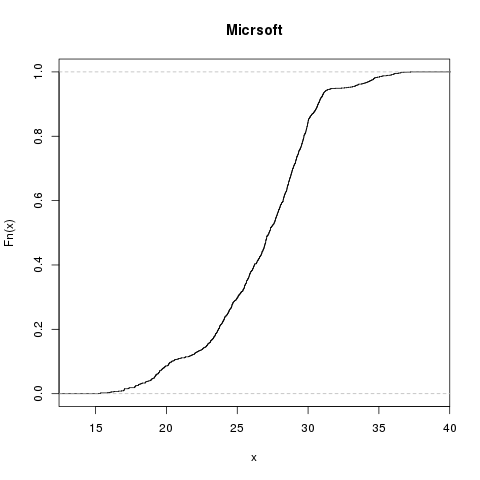
\includegraphics[scale=0.75]{RPlotExample.png}
 
\subsubsection{Documentation quality and quantity}
In comparison to Python, R was build solely for analytical purposes. Since the language was build for analysis by the scientific community R's documentation is built in a scientific manner. To evaluate the documentation we will use the points system described in the Python Documentation section.\\
The R Base package:
\begin{enumerate}
    \item 1 Point (the documentation was available during the whole time of the program development).
    \item 0 Points (the navigation is alphabetic).
    \item 0 Points (the native documentation does not provide a sufficient amount of examples).
    \item 0.5 Points.
    \item 0 Points.
    \item 1 Points.
    \item 0 Points (no styling was applied).
\end{enumerate}
The Stats package is organized in a similar way to the base R package and have the similar score:
\begin{enumerate}
    \item 1 Point.
    \item 0 Point (the alphabetical list with short description).
    \item 0.5 Points.
    \item 0.5 Points.
    \item 0 Point.
    \item 1 Point.
    \item 0 Points (no styling applied).
\end{enumerate} 
The Nlme package is hosted by the biggest R source called "CRAN". This source offers a significant amount of simple and complex demos, test data sets and tutorials. CRAN is considered to be the central R source.
\begin{enumerate}
    \item 1 Point.
    \item 1 Point (the documentation is organized as a scientific paper with the content provided).
    \item 1 Point.
    \item 1 Point.
    \item 0 Points.
    \item 1 Point (the theoretical background is provided in the form of the references after the function explanation).
    \item 1 Point (scientific paper formatting).
\end{enumerate}
The last package used in our program is Tseries:
\begin{enumerate}
    \item 1 Point (hosted by CRAN).
    \item 1 Point (scientific paper).
    \item 1 Points.
    \item 1 Point.
    \item 0 Point.
    \item 1 Point.
    \item 1 Point.
\end{enumerate}
The quality of the R documentation is on average on the same level for all sources. However the convenience of the documentation differs depending on the source and the development team. The total score for the R documentation is:
\[ \frac{\frac{3}{10}(2.5)+\frac{1}{10}(3)+\frac{3}{10}(6)+\frac{3}{10}(6)}{7}= 0.66 \] 

\subsubsection{Advantages And Disadvantages Of The Program}
During the development phase of our second program we have encountered several difficulties associated with the language features. Since we have already written our program in Python we have decided to implement the same structure.\\
The first advantage of the R program is the data frame object and correlated functions. The performance of the slicing and formatting operations is good. One of the most useful functions during the work with R data objects was str(). This function shows the structure of the object:
\begin{verbatim}
> str(data)
'data.frame':   1239 obs. of  69 variables:
 $ Intel                : num  26.6 26.6 26.4 25.8 25.9 ...
 $ AMD                  : num  27.5 28.4 27.8 27.9 29.2 ...
 $ Qualcomm             : num  46.5 45.6 45.4 43.8 44.2 ...
 $ MicronTech           : num  13.5 13.6 13.6 13.6 13.9 ...
 $ Infenion             : num  9.26 9.38 9.41 9.3 9.25 9.23 9.21 9.23 9.26 9.19 ...
 $ STMElectro           : num  18.5 18.7 18.6 18.1 18.2 ...
...
\end{verbatim}
There are several language specific functions to extract the sub data from the original data frame. For example, to get all the companies names from the table you can use colnames():
\begin{verbatim}
> names <- colnames(data)
> class(names)
[1] "character"
> str(names)
 chr [1:69] "Intel" "AMD" "Qualcomm" "MicronTech" "Infenion" ...
\end{verbatim} 
In the Python program where we had to store the data into the dictionary with the names as the keys and the lists of share prices as the associated values. In R the names of the companies from the data frame are coming in exact same order as they appear in the csv file.\\
The second advantage of the R program is connected to the the function we have used for the regression building. As we have described in the Program Structure and Used Libraries sections for the regression we have used gls function from the nlme package. In order to use this function the formula for the regression and the data containing all given names from the formula should be provided. Two examples of the gls use are presented below (the following examples are not the optimal decision):
\begin{verbatim}
> model1<-gls(Intel ~ Olympus + Google + AMD + St.Jude, data)
> model1
Generalized least squares fit by REML
  Model: Intel ~ Olympus + Google + AMD + St.Jude 
  Data: data 
  Log-restricted-likelihood: -1959.999

Coefficients:
(Intercept)     Olympus      Google         AMD     St.Jude 
-1.38174717  0.18731627  0.01450565  0.05510854  0.21830586 

Degrees of freedom: 1239 total; 1234 residual
Residual standard error: 1.158712
>
> model2<-gls(Intel ~ sin(pi*Olympus) + cos(2*pi*AMD) + St.Jude, data)
> model2
Generalized least squares fit by REML
  Model: Intel ~ sin(pi * Olympus) + cos(2 * pi * AMD) + St.Jude 
  Data: data 
  Log-restricted-likelihood: -2875.022

Coefficients:
      (Intercept) sin(pi * Olympus) cos(2 * pi * AMD)           St.Jude 
       1.78264194        0.19693369        0.03505161        0.46976204 

Degrees of freedom: 1239 total; 1235 residual
Residual standard error: 2.451844
\end{verbatim}
Another advantage of the gls function is its data use. In comparison to Python the data is not required to be specifically formatted. The data frame previously loaded into the environment will be used by default if no data is specified. If there are more than one data sources loaded into the environment the specification is not optional.\\
The third advantage of the R program is its performance. Without using the explicit multiprocessing or JIT the program has significantly outperformed the Python program. The actual results will be presented in the following section.\\
The first disadvantage of the R language is difficulty. The syntax is not as intuitive as the Python syntax. The data structures and their use are non trivial. In order to begin using R significant amount of time invested upfront is needed. The R background of the author of this work consisted of the basic programming course [20] using RStudio [21]. RStudio is a good IDE for R to begin with. However it limits the development freedom for the complex tasks.\\
The first example of the R complexity is the absence of the classes in their usual understanding. In R there are three type of classes. These are S3, S4 and Reference Class. The reference class is close to the Python class. The first two represent the attribute of an object. In R everything considered as an object. In our program we have used the reference class and didn't dive into the other two class types. For more information on OO systems in R you can visit the following source [22]. \\
The second disadvantage of the R program is connected to Reference Class definition. In R the return statement with multiple instances is not allowed. Following example shows the wrong implementation. It will return an error:
\begin{verbatim}
getData <- setRefClass("getData",
    fields = list( name="character", data="data.frame", companies="character"),
	methods = list( 
    	get_data = function() {
            data <<- read.csv(name, header = TRUE, sep = ",", 
            quote = "\"", dec = ".", fill = TRUE, comment.char = "")
			companies <<- colnames(data)
			
			return data, companies
		})
\end{verbatim}
In order to be able to return several objects it is possible to write them down into a list:
\begin{verbatim}
getData <- setRefClass("getData",
    fields = list( name="character", result="list"),
	methods = list( 
    	get_data = function() {
            data <- read.csv(name, header = TRUE, sep = ",", 
            quote = "\"", dec = ".", fill = TRUE, comment.char = "")
			companies <- colnames(data)
            
            result <<- c(data, result)
            result<<- c(companies, result)
            
            return result            			
		})
\end{verbatim}
The disadvantage of this workaround is the additional formatting of the resulting list:
\begin{verbatim}
> d <- getData(name="../data/LearningSet.csv")
> result <- d$get_data()
>class(result)
[1] "list"
> data <- result[[1]]
> companies <- result[[2]]
\end{verbatim}
Another disadvantage of the R program in is the difficulty of the slicing. Different approaches can be used to get the same result. However there are several difficulties connected with some approaches. The following example shows different approaches to print out the first five prices of the Intel:
\begin{verbatim}
> data$Intel[1:5]
[1] 26.59 26.58 26.37 25.80 25.85
> class(data$Intel[1:5])
[1] "numeric"
>
> data[[1]][1:5]
[1] 26.59 26.58 26.37 25.80 25.85
> class(data[[1]][1:5])
[1] "numeric"
>
> data[names(data)[1]][[1]][1:5]
[1] 26.59 26.58 26.37 25.80 25.85
> class(data[names(data)[1]][[1]][1:5])
[1] "numeric"
>
> data[,1][1:5]
[1] 26.59 26.58 26.37 25.80 25.85
> class(data[,1][1:5])
[1] "numeric"
\end{verbatim}

\subsection{Results}
The main file implemented in the R program consists of two functions using implemented classes. The first function activates the libraries we have used in the program and calls the implemented classes in a specific order. The output is printed to the terminal. The extended information on the resulting regression is called separately to the result output for the gls function:
\begin{verbatim}
> source("main.r")
> system.time(main())
[1] "The parameters limit is not reached, searching further"
[1] "The parameters limit is not reached, searching further"
[1] "The parameters limit is not reached, searching further"
[1] "The parameters limit is not reached, searching further"
Generalized least squares fit by REML
  Model: as.formula(form[[k1]]) 
  Data: data 
       AIC      BIC    logLik
  3421.976 3462.907 -1702.988

Coefficients:
                Value  Std.Error   t-value p-value
(Intercept)  4.588765 0.29835356  15.38029       0
Cardinal    -0.073992 0.00540346 -13.69342       0
Olympus      0.054461 0.01080308   5.04127       0
St.Jude      0.165351 0.00801178  20.63845       0
Lenovo       0.500866 0.01499778  33.39599       0
MicronTech   0.073363 0.01235370   5.93858       0
STMElectro   0.435386 0.02655304  16.39685       0

 Correlation: 
           (Intr) Cardnl Olymps St.Jud Lenovo McrnTc
Cardinal   -0.208                                   
Olympus    -0.492  0.210                            
St.Jude    -0.846 -0.113  0.212                     
Lenovo      0.447 -0.046 -0.834 -0.408              
MicronTech -0.421  0.252  0.267  0.273 -0.180       
STMElectro  0.494 -0.802 -0.590 -0.203  0.415 -0.614

Standardized residuals:
       Min         Q1        Med         Q3        Max 
-2.3116653 -0.7048518 -0.0818459  0.6500465  3.5270072 

Residual standard error: 0.9389829 
Degrees of freedom: 1239 total; 1232 residual


   user  system elapsed 
 24.566   0.000  23.461 

\end{verbatim}    
The best model returned by the R program consist of 6 companies. These companies are STMElctro, Olympus, St.Jude, Lenovo, Microntech and Cardinal. The R program has chosen Cardinal over Google on the last step of the evaluation algorithm. Since the programs are identical this deviation can be caused by the underlying implementations of the gls function, the llr test, or the AIC criterion evaluation. Since we didn't found the source code for the functions we have used in this work, the cause of the difference in the results can't be explained properly. To compare the results of the programs we have built the predictions for both programs. First the accuracy of the original predictions will be compared. Afterwards the cross results accuracy will be compared. The program yielding the higher accuracy predictions will get an additional point.\\
To sum up the objective arguments for R we will give the points according to the evaluation table given in the description section. The Points for the R program are:
\begin{enumerate}
    \item Useful sources: 1 Point.
    \item Documentation: 0.66 Points.
    \item Performance: 1 Point.
    \item Memory: 1 Point.
    \item Uniform data structures: 1 Point.
    \item Big Data: 1 Point (this is a relatively recent addition to the language. There are several sources and libraries offering tools to work with big data [23]).
    \item Visualization: 1 Point.
    \item Limitations: 1 Point (high complexity of the language).
    \item Workarounds: 1 Point.
\end{enumerate} 
The total objective score for R is 7.66 points total.\\
The subjective arguments for the language are:
\begin{enumerate}
    \item Debugging messages are hard to understand.
    \item Certain amount of time is needed to understand the code since the syntax is not intuitive.
    \item Layered structures were confusing.
    \item No additional formatting saved time.
    \item More.
\end{enumerate}

\newpage
\section{Results}
In this section we will present the final comparison of the programs written in Python and R.

\subsection{Objective comparison}
The first difference between the programs is the performance. In order to show measure the run time of the programs we will use the options that both language offer. These methods are system.time() for R and cProfile() for Python. Additionally to the language specific functions we will use the /bin/time linux utility. Th following example shows us the run time for the R program.
\begin{verbatim}
> system.time(data_read())                                                                  
   user  system elapsed                                                                       
  0.100   0.000   0.085  
> system.time(stat(build_data, companies))
   user  system elapsed 
  3.627   0.000   3.465
>> system.time(model(build_data, companies, rest, dependent))
   user  system elapsed 
  3.837   0.000   3.067 
\end{verbatim}
The main function consists of three parts. The first part reads the data from the csv table and formats it. The second part runs statistic tests. The third part buildings a model based on the results of the statistic tests. The overall time of the program can be measured via main and predict functions:
\begin{verbatim}
> system.time(main())
   user  system elapsed 
  8.917   0.000   6.546 
> system.time(build_predictions())
[1] "the mean of the y is: "
[1] 23.46462
[1] "the std of the y is: "
[1] 2.55532
[1] "the mean of the predictions is: "
[1] 20.86923
[1] "the std of the predictions is: "
[1] 1.544088
   user  system elapsed 
  0.000   0.000   0.117 
\end{verbatim}
The run time of the main function is greater than the sum of its parts, since the main function loads needed libraries and also counts the time for the data transfer between the classes as well as the initialization of the classes. The Python program performance in our implementation is 750 times slower. R program runs for 7.41 seconds versus 5564.19 seconds Python program.\\
\textcolor{red}{rython crofile results}\\
The second difference between the programs is the memory usage. There are several possibilities to measure the memory load of the program. Since every instance in R is treated as an object the size of all objects can be shown using Rprofmem() function from the utilities package. However, in order to use this function to compute the total memory use the sum of the all ojects size needs to be computed. This approach is complex and does not guarantees the accurate result. Python also offers different tools to do the profiling. On of the possible functions is memory\_profile [11]. In order to measure the memory use uniformly for both languages we will use the unix time command. The printed message contains the information about the called process. Two main characteristics we are interested in are the maximum resident set size and the user time. The maximum resident set size shows the amount of the memory belogning to the process and currently presented in RAM. In aother words it is the maximum memory allocated in the heap by the program.\\ 
The R memory use looks as following:
\begin{verbatim}
[20:32:19 - 15-10-25] 
/home/alisa/uni-stuff/Bachelor/r % /usr/bin/time -v R  main.r
        Command being timed: "R main.r"
        User time (seconds): 7.41
        System time (seconds): 0.05
        Percent of CPU this job got: 18%
        Elapsed (wall clock) time (h:mm:ss or m:ss): 0:41.45
        Average shared text size (kbytes): 0
        Average unshared data size (kbytes): 0
        Average stack size (kbytes): 0
        Average total size (kbytes): 0
        Maximum resident set size (kbytes): 78436
        Average resident set size (kbytes): 0
        Major (requiring I/O) page faults: 0
        Minor (reclaiming a frame) page faults: 17697
        Voluntary context switches: 59
        Involuntary context switches: 2026
        Swaps: 0
        File system inputs: 0
        File system outputs: 2840
        Socket messages sent: 0
        Socket messages received: 0
        Signals delivered: 0
        Page size (bytes): 4096
        Exit status: 0
\end{verbatim}
The maximum memory usage of the R program is 78,4 MB.\\
The Python memory use looks as following:
\begin{verbatim}
[19:11:27 - 15-10-25] 
/home/alisa/uni-stuff/Bachelor/python % /usr/bin/time -v python __main___.py
        Command being timed: "python __main___.py"
        User time (seconds): 5564.19
        System time (seconds): 7.73
        Percent of CPU this job got: 100%
        Elapsed (wall clock) time (h:mm:ss or m:ss): 1:32:46
        Average shared text size (kbytes): 0
        Average unshared data size (kbytes): 0
        Average stack size (kbytes): 0
        Average total size (kbytes): 0
        Maximum resident set size (kbytes): 637036
        Average resident set size (kbytes): 0
        Major (requiring I/O) page faults: 0
        Minor (reclaiming a frame) page faults: 3633280
        Voluntary context switches: 3047
        Involuntary context switches: 22080
        Swaps: 0
        File system inputs: 0
        File system outputs: 8976
        Socket messages sent: 0
        Socket messages received: 0
        Signals delivered: 0
        Page size (bytes): 4096
        Exit status: 0
\end{verbatim}
The maximum memory usage of the Python program is 637,0 MB.\\
As we have mentioned earlier, we will compare the predictions of the programs and evaluate the cross results. The predictions were built on the TestingSet file containing 515 prices for the time period from 1.01.2011 to 31.12.2012. We will show the main characteristics of the predictions row: mean and standard deviation as well as the comparison plot.\\
The R program gives us following results:
\begin{verbatim}
> p<-build_predictions()
[1] "the mean of the y is: "
[1] 23.46462
[1] "the std of the y is: "
[1] 2.55532
[1] "the mean of the predictions is: "
[1] 20.86923
[1] "the std of the predictions is: "
[1] 1.544088
[1] "the mean absolute error of the predictions is: "
[1] 3.29319
[1] "the root mean squared error of the predictions is: "
[1] 4.132798
\end{verbatim}
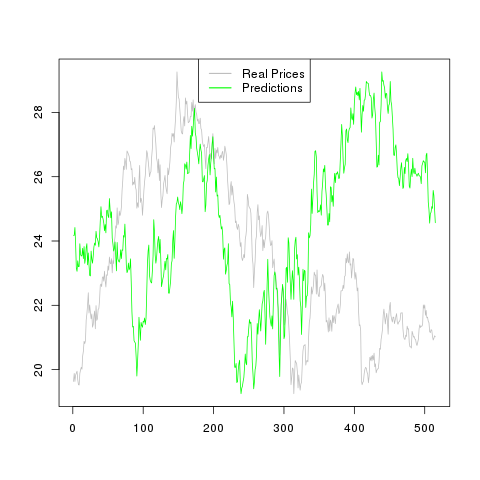
\includegraphics[scale=0.75]{RPredicitions.png}
The Python program results are:
\begin{verbatim}
>>> build_predictions()
the mean of the y is: 23.4646213592
the std of the y is: 2.55283813168
the mean of the prediction is: 21.8848266352
the standard deviation is: 1.35949376438
the mean absolute error of the prediction is: 2.83819120505
the root mean squared error is: 3.47169327209
\end{verbatim}
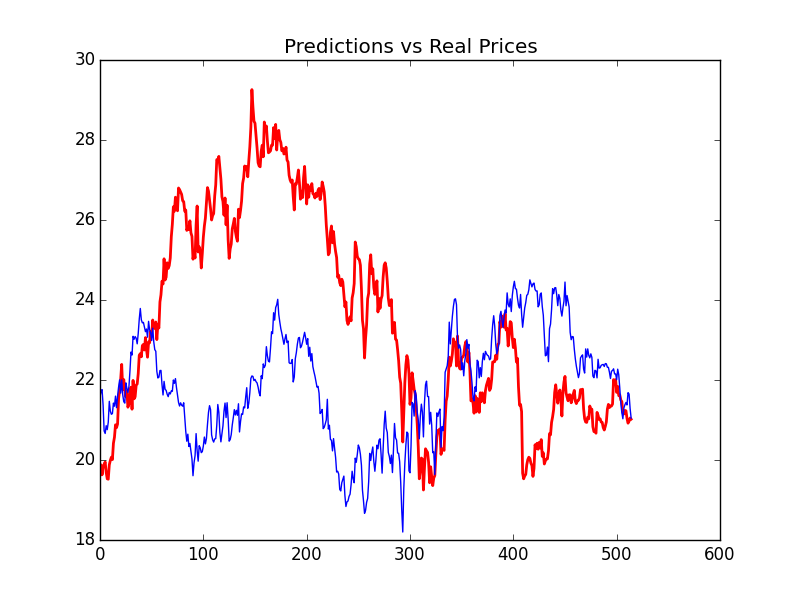
\includegraphics[scale=0.75]{PythonPredictions.png}\\
The Python predictions according to the chosen criteria are more accurate than the R predictions. Both mean absolute error (MAE) and root mean square error (RMSE) are smaller for the Python predictions. The Python program gets one additional point for the relative accuracy. On the following graph both original R and Python predictions are shown. The R forecasts have the green line and the blue line presents the Python forecasts.\\
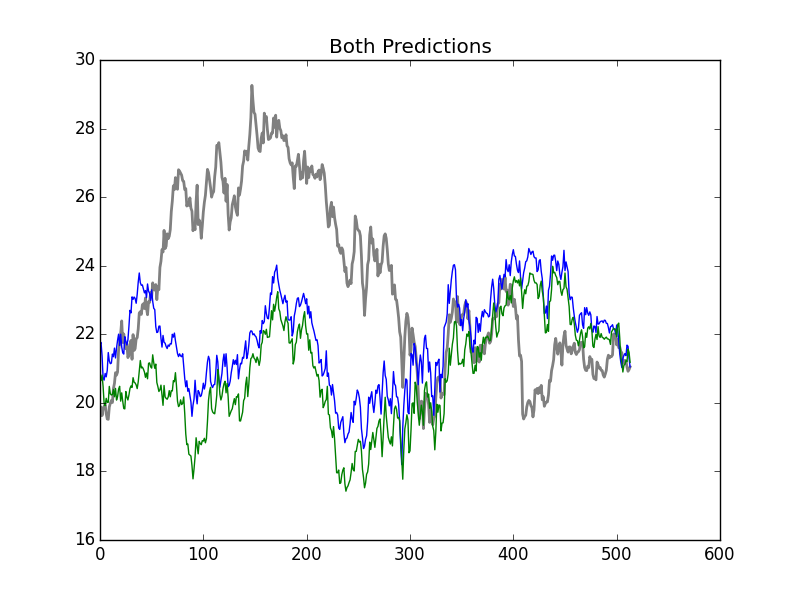
\includegraphics[scale=0.75]{BothPredictions.png}\\
As the following step we will force both Python and R programs to compute the results for the model yielded by the other program. Python will compute predictions for the final model from R: ["Cardinal", "Olympus", "St.Jude", "Lenovo", "MicronTech", "STMElectro"]. And the R program will return the forecast for the Python final model: ["Google", "Olympus", "St.Jude", "Lenovo", "MicronTech", "STMElectro"]\\
The R cross result is:
\begin{verbatim}
> p<-build_predictions()
[1] "the mean of the y is: "
[1] 23.46462
[1] "the std of the y is: "
[1] 2.55532
[1] "the mean of the predictions is: "
[1] 21.73608
[1] "the std of the predictions is: "
[1] 1.152263
[1] "the mean absolute error of the predictions is: "
[1] 2.631951
[1] "the root mean squared error of the predictions is: "
[1] 3.305496
> p$model
Generalized least squares fit by REML
  Model: Intel ~ Olympus + Google + St.Jude + MicronTech + STMElectro +      Lenovo 
  Data: build_data 
  Log-restricted-likelihood: -1760.532

Coefficients:
(Intercept)     Olympus      Google     St.Jude  MicronTech  STMElectro 
2.299629176 0.047291974 0.005870799 0.165562665 0.105875773 0.167784354 
     Lenovo 
0.401918284 

Degrees of freedom: 1239 total; 1232 residual
Residual standard error: 0.982245 
\end{verbatim}
On the following image the difference in two models forecasts returned by the R program is represented. The gray line shows the real Intel prices, the green line is the new model forecast and the blue line is the old model forecast.\\
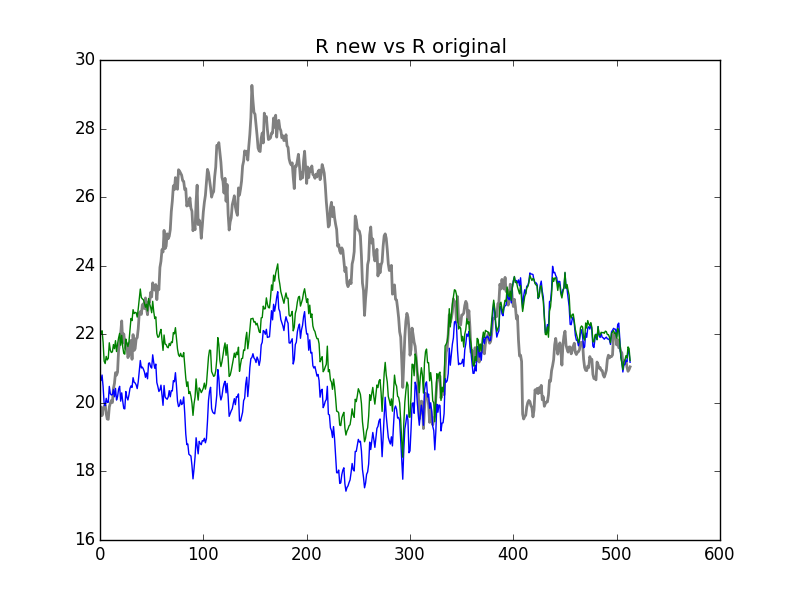
\includegraphics[scale=0.75]{ROriginalVsNew.png}\\
The R program considers the new model to be better than the original suggestion since the new MAE is 0.661 smaller and the new RMSE is 0.827 smaller. The original model was chosen based on the AIC. The forecast was built only for the final model. That means that we never considered the accuracy of the predictions as the criterion for thoosing the best model in the class or among two classes.\\
The following graph represents the predictions for the same model but estimated by different program. The model is ["Google", "Olympus", "St.Jude", "Lenovo", "MicronTech", "STMElectro"]. As usual the gray line presents the real values, the green line is the R forecast, the blue line is the Python forecast.\\
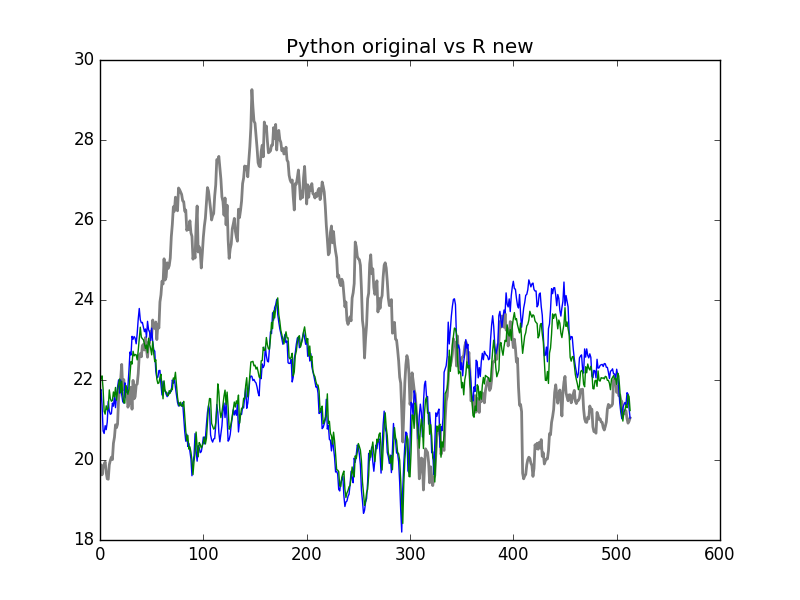
\includegraphics[scale=0.75]{PythonOriginalVsRNew.png}
we have noticed that the predictions built by the R program for the Python original model have higher accuracy than the Python predictions for the same model. The R MAE is 0.208 smaller and the R RMSE is 0.166 smaller than the Pyhton results.
The Python cross results are:
\begin{verbatim}
>>> build_predictions()
the mean of the y is: 23.4646213592
the std of the y is: 2.55283813168
the mean of the prediction is: 20.699905831
the standard deviation is: 2.18673197501
the mean absolute error of the prediction is: 3.9100716967
the root mean squared error is: 4.81718549588

the model is: ['STMElectro', 'Olympus', 'St Jude', 'Lenovo', 'MicronTech', 'Cardinal']
                            GLS Regression Results                            
==============================================================================
Dep. Variable:                      y   R-squared:                       0.998
Model:                            GLS   Adj. R-squared:                  0.998
Method:                 Least Squares   F-statistic:                 8.261e+04
Date:                Mon, 26 Oct 2015   Prob (F-statistic):               0.00
Time:                        14:34:25   Log-Likelihood:                -1785.4
No. Observations:                1239   AIC:                             3583.
Df Residuals:                    1233   BIC:                             3613.
Df Model:                           6                                         
Covariance Type:            nonrobust                                         
==============================================================================
                 coef    std err          t      P>|t|      [95.0% Conf. Int.]
------------------------------------------------------------------------------
x1             0.2337      0.025      9.273      0.000         0.184     0.283
x2             0.1363      0.010     13.277      0.000         0.116     0.156
x3             0.3977      0.015     27.166      0.000         0.369     0.426
x4            -0.0567      0.006     -9.826      0.000        -0.068    -0.045
x5             0.2696      0.005     57.903      0.000         0.261     0.279
x6             0.1533      0.012     12.533      0.000         0.129     0.177
==============================================================================
Omnibus:                       32.097   Durbin-Watson:                   0.140
Prob(Omnibus):                  0.000   Jarque-Bera (JB):               18.122
Skew:                           0.114   Prob(JB):                     0.000116
Kurtosis:                       2.453   Cond. No.                         70.4
==============================================================================
\end{verbatim}
The following graph shows the difference between two models forecasts returned by the Python program. The gray line shows the real values, the green line presents the new model forecast and the blue line is the old model forecast.\\
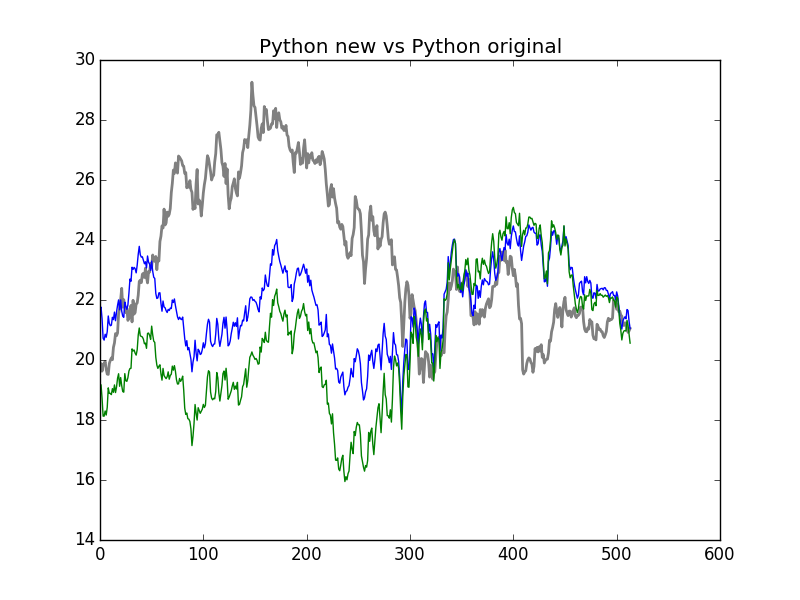
\includegraphics[scale=0.75]{PythonOriginalVsPythonNew.png}\\
The Python program considers the new model to be worse in comparison to the original suggestion since the MAE is 1.072 smaller and the RMSE is 1.4 smaller than the original results. The first Python model was chosen based on the AIC and the predictions were also not taken into account during the evaluation steps.\\
The following graph presents the predictions for the same model but estimated by different program. the model is ["Cardinal", "Olympus", "St.Jude", "Lenovo", "MicronTech", "STMElectro"]. Same color notation is used.\\
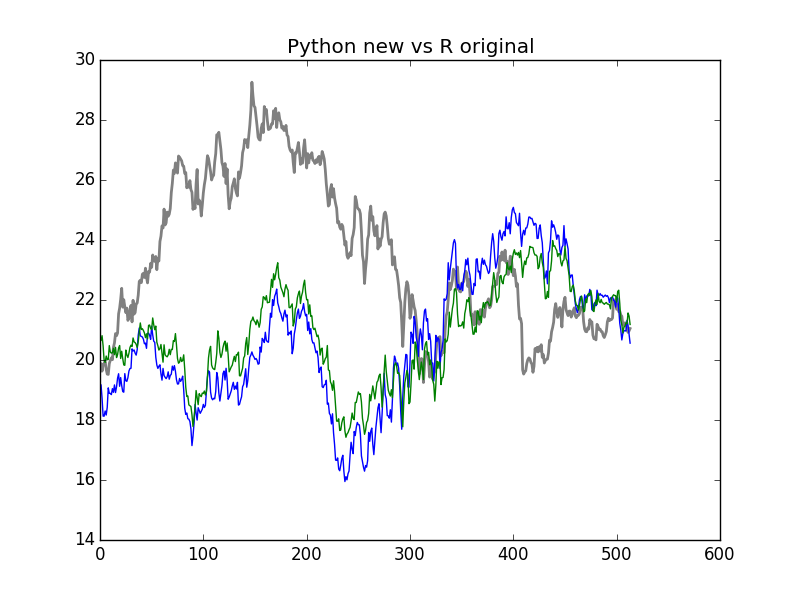
\includegraphics[scale=0.75]{ROriginalVsPythonNew.png}
The Python program predictions are less accurate than the R predictions for the same model. The R MAE is 0.617 smaller and the R RMSE is 0.684 smaller.\\
The higest accuracy forecast was built by the R program for the Python original model. This result can be explained by the fact that R gls.predict() module uses higher accuracy computation algorithm and operates with doubles insaead of floats. At the same time the Python program has returned better regression using the AIC during the evaluation process. Python gets an additional Point for yielding higher accuracy results.\\
The final score for both programs is 7.66 Points for the R program versus 6.71 Points for the Python program. This mean that objectively R is more suitable for beginners to use as the programming language for a small statistic task with a small data set.

\subsection{Subjective comparison}
During the process of the program development both languages have shown some of their advantages and disavantages. The subjective advantages of the Python are:
\begin{enumerate}
    \item Easy code refactoring.
    \item Sufficient amount of tutorials and examples for every function used in the program.
    \item Intuitive data structures.
    \item Clear debugging messages.
    \item Possibility to use a simple speed up in the form the of the pypy.
\end{enumerate}
The subjective disadvantages of the language are:
\begin{enumerate}
    \item Slow third-party functions for statistic tests.
    \item Formatting step a lot of time to implement.
    \item The Pandas library does not work with the pypy interpreter.
\end{enumerate} 
The R program subjective disadvantages encountered during the program development are:
\begin{enumerate}
    \item The run time.
    \item Data structures are easy to use.
    \item Low memory allocation.
\end{enumerate}
The subjective diasdvantages of the language are:
\begin{enumerate}
    \item Non intuitive syntax.
    \item Difficultie while calling R code outside of the runtime.
    \item Not enough examples for the functions usage.
\end{enumerate} 
Subjectively speaking R is slightly better for the data analysis programs when the program architecture was already specified. For the higher complexity programs R will be more suitable than Python.\\ 
Python proved to be more suitable for a fast prototyping using a small data set. Another advantage of the Python program is the absence of the integration necessity.
  
\subsection{Conclusion}
After point to point comparison and collecting the personal opinion, we have decided, that R programming language is more suitable for pure analytical task.
\begin{enumerate}
    \item The language is faster.
    \item The language is not memory hungry.
    \item The results are adequately accurate. 
    \item The complex functions are easier to use.
\end{enumerate}
The R language has a big high-quality community behind it. There are certain standards for the documentation and the code quality, which ensures the quality of the libraries.\\
The negative moment can be the development of a bigger program. Prototyping in R can be tricky for mid- and very complex programs. You have to think in advance about class connections. Although you can also keep everything in functions form - this will allow you to prototype faster, but will cause some difficulties later on during refactoring.\\
  

\newpage
\section{Literature}
\begin{enumerate}
    \item \url{https://en.wikipedia.org/wiki/Python_(programming_language)}
    \item \url{https://www.digitalocean.com/community/tutorials/how-to-package-and-distribute-python-applications}
    \item \url{https://www.r-project.org/about.html}
    \item \url{http://www.revolutionanalytics.com/what-r}
    \item \url{https://en.wikipedia.org/wiki/R_(programming_language)}
    \item \url{http://stackoverflow.com/questions/2770030/r-or-python-for-file-manipulation}
    \item \url{http://datascience.stackexchange.com/questions/326/python-vs-r-for-machine-learning}
    \item \url{http://www.kdnuggets.com/2015/05/r-vs-python-data-science.html}
    \item \url{http://blog.datacamp.com/r-or-python-for-data-analysis/}
    \item \url{http://101.datascience.community/2015/05/12/data-science-wars-r-vs-python/}
    \item Memory Profiler for Python \url{https://github.com/fabianp/memory_profiler} 
    \item Python 3 \url{https://www.python.org/doc/}
    \item SciPy \url{http://www.scipy.org/}
    \item Statmodels \url{http://statsmodels.sourceforge.net/}
    \item Six \url{https://pythonhosted.org/six/}
    \item Base R library \url{https://stat.ethz.ch/R-manual/R-devel/library/base/html/00Index.html}
    \item Stats R library \url{https://stat.ethz.ch/R-manual/R-patched/library/stats/html/00Index.html}
    \item Nlme R library \url{https://cran.r-project.org/web/packages/nlme/nlme.pdf}
    \item Tseries R library \url{https://cran.r-project.org/web/packages/tseries/tseries.pdf}
    \item Coursera: "R Programming"\url{https://www.coursera.org/course/rprog}
    \item RStudio IDE \url{https://www.rstudio.com/}
    \item OO systems in R \url{http://adv-r.had.co.nz/OO-essentials.html}
    \item Big Data in R \url{http://r-pbd.org/}
    \item GLS \url{https://en.wikipedia.org/wiki/Generalized_least_squares}
\end{enumerate}
\end{document}